\documentclass[conference]{IEEEtran}
\IEEEoverridecommandlockouts

\usepackage{cite}
\usepackage{amsmath,amssymb,amsfonts}
\usepackage{graphicx}
\usepackage{booktabs}
\usepackage{xcolor}
\usepackage{url}
\usepackage{placeins}
\usepackage{float}
\usepackage[hidelinks]{hyperref}

% ── Compact macros for the moment quantities ─────────────────────────────
\newcommand{\mt}{m(t)}
\newcommand{\mhat}{\hat m(t)}
\newcommand{\mbar}{\bar m(t)}
\newcommand{\eps}{\varepsilon}
\newcommand{\epstwo}{\varepsilon_2}

\begin{document}

\title{A Physics-Informed Neural Network Framework for\\
Predicting Dynamics of Ising-Like Zimm-Bragg Systems}

\author{
  \IEEEauthorblockN{Meruzhan Khachatryan}
  \IEEEauthorblockA{
    BS in Data Science\\
    American University of Armenia\\
    Yerevan, Armenia\\
    Supervisor: Varazdat Stepanyan\\
    Email: \href{mailto:meruzhan_khachatryan@edu.aua.am}{meruzhan\_khachatryan@edu.aua.am}
  }
}

\maketitle

\begin{abstract}
The Zimm-Bragg model captures the cooperative helix-coil transition in
polypeptides through the same mathematical structure as a one-dimensional
Ising chain under Glauber dynamics. Predicting its time evolution is
typically done with Monte Carlo simulation (physically faithful but
expensive) or with black-box neural networks (fast but unconstrained by the
underlying physics). I propose a Physics-Informed Neural Network (PINN)
framework that bridges the two by embedding the closed-moment Glauber
ordinary differential equations directly in the training loss. A single
small multilayer perceptron is trained to fit the helicity trajectory
$\mbar$, while three trainable scalars play the role of the Glauber
coefficients $(a_0, a_1, a_2)$. The two correlation functions
$\eps(t)$ and $\epstwo(t)$ are then recovered analytically without any
additional networks or supervision. Across a 100-condition grid in
$(\beta, h, J)$, the PINN reproduces the Monte Carlo trajectories with mean
squared error on the order of $10^{-7}$ on the helicity and matches
the analytical Glauber forward map to within $\sim\!10^{-3}$ on the
recovered coefficients. I benchmark the chosen design against four
alternative PINN variants (separate-channel, inverse, 3-channel, per-run)
and find that the analytical post-hoc reduction is the most
parameter-efficient and most stable of the candidates considered. The
result is a compact surrogate for the chain's full dynamics that respects
the governing equations by construction.
\end{abstract}

\section{Introduction}
\label{sec:intro}

A wide range of systems in physics, chemistry, and biology share a common
mathematical skeleton: a lattice of two-state variables that interact only
with their nearest neighbors, controlled by an external bias and a
temperature. The Ising model is the first such model and it was made to describe
ferromagnetism.~\cite{landau-stat}. A modification of the 1d ising model is the Zimm-Bragg model
 of helix-coil transitions in polypeptides.~\cite{zimmbragg1959}. In both cases, the dynamics of the
system at finite temperature are captured by Glauber single-spin-flip
updates, whose macroscopic average is approximately described by a closed system of
ordinary differential equations (ODEs) for the helicity and short-range
correlators~\cite{glauber1963,allahverdyan2009kinetics}.

Predicting the time evolution of such systems today involves a trade-off.
Monte Carlo simulation reproduces the underlying physics exactly but is
expensive at scale, particularly when many conditions must be swept or
when long trajectories are required for relaxation studies. Black-box
neural networks can be orders of magnitude faster at inference time, but
nothing in their training loss prevents them from violating the governing
equations of motion: small perturbations in the data can lead to
predictions that are not even physically admissible.

Physics-Informed Neural Networks (PINNs) are an emerging framework that
attempts to bridge this gap by penalizing violations of the underlying
ODEs or PDEs directly in the training loss~\cite{raissi2019pinn}. Most
PINN literature targets continuous-field problems (fluids, elasticity,
heat transfer); applications to discrete spin systems are still comparatively underexplored.
The closed-moment Glauber description of an Ising-like chain is
particularly well suited to a PINN treatment because the macroscopic
dynamics close into a low-dimensional ODE system whose right-hand side is
parameterized by three scalar coefficients.

This work develops and benchmarks a PINN framework for that setting. The
specific contributions are:

\begin{enumerate}
  \item A compact PINN architecture that learns the helicity
    trajectory $\mhat$ together with the three Glauber coefficients
    $(a_0, a_1, a_2)$ from a single observed trajectory.
  \item A closure-free analytical post-hoc step that recovers the
    nearest-neighbor and next-nearest-neighbor correlators
    $\eps(t)$ and $\epstwo(t)$ from the trained model, without any
    additional supervision.
  \item A head-to-head benchmark against four alternative PINN variants
    (three-separate-channel, inverse, 3-channel, and per-run), which
    isolates the design choices that matter for accuracy and stability.
  \item A demonstration that the proposed pipeline matches the
    Monte Carlo ground truth to high precision across a 100-condition
    parameter grid, while recovering the underlying Glauber coefficients
    to within $\sim\!10^{-3}$.
\end{enumerate}

The remainder of the paper proceeds from background to method to results.
 It begins by placing the contribution in context, reviewing PINNs, the 
 closed-moment description of Glauber dynamics, and prior machine-learning 
 work on spin systems. It then formulates the closed-moment system and presents
  the PINN architecture, training procedure, and data pipeline, followed by
   experimental results, a validation against Monte Carlo ground truth and
   four alternative PINN variants, and a concluding discussion.

\section{Literature Review}
\label{sec:litreview}


The Ising model~\cite{landau-stat} describes a lattice of binary spins
$\sigma_i \in \{-1, +1\}$ that interact via a nearest-neighbor coupling
$J$ and are biased by an external field $h$, in thermal equilibrium at
inverse temperature $\beta = 1/k_B T$. Its one-dimensional version is
analytically solvable and exhibits no finite-temperature phase transition,
but the model has remained influential because the same
structure recurs in widely different physical contexts. In the
biophysical context studied by Zimm and Bragg~\cite{zimmbragg1959}, each
spin represents the conformational state of an amino acid residue
($+1$ for $\alpha$-helix, $-1$ for random coil), the coupling $J$
represents the cooperativity of helix propagation along the chain, and
the field $h$ aggregates helix preferences and environmental
factors. Recent work by Stepanyan et al.~\cite{stepanyan2024} has revisited
the finite-size thermal transitions of the one-dimensional Ising chain,
which is the system the experiments here target. The corresponding
kinetics of the Zimm-Bragg chain under finite-rate temperature
changes have been studied by Allahverdyan et
al.~\cite{allahverdyan2009kinetics}, who derive the closed-moment
ODE system used throughout this paper and document its hysteresis
and memory behavior under non-equilibrium driving.


Equilibrium statistical mechanics fixes only the long-time distribution
of spin configurations; the dynamical relaxation toward equilibrium
requires a separate prescription. Glauber dynamics~\cite{glauber1963}
provide such a prescription: at each step, a single spin is selected at
random and is flipped with a probability given by the local
Monte-Carlo rule. The macroscopic averages of single-spin and pair
observables under Glauber dynamics satisfy a coupled system of ODEs that
can be expanded in low-order moments. Allahverdyan et
al.~\cite{allahverdyan2009kinetics} derive this expansion explicitly
for the Zimm-Bragg chain in non-zero field and use it to study the
helix-coil kinetics under finite-rate temperature changes. For the
1D Ising chain, the expansion closes at the level of
$(m, \eps, \epstwo)$ with three composite coefficients
$(a_0, a_1, a_2)$ that are functions of $(\beta, h, J)$ via a tanh
forward map~\cite{landau-stat,allahverdyan2009kinetics}.


PINNs were introduced by Raissi, Perdikaris and Karniadakis as a way to
integrate governing equations into the training of deep
networks~\cite{raissi2019pinn}. The key idea is that the loss function
combines a data-fitting term with a residual term that penalizes
violations of the governing ODE/PDE evaluated at random collocation points,
where derivatives of the network output are computed by automatic
differentiation. This framework has since been applied to a broad range of
forward and inverse problems in continuous media, but applications to
discrete spin systems and Glauber-type dynamics are comparatively rare.
The present work extends the PINN framework to that setting by using the
closed-moment Glauber ODE as the physics constraint.


Independent of the PINN line of work, there is a body of literature on
applying neural networks to Ising-type systems for tasks such as
configuration generation, equilibrium-property prediction, and order-parameter
identification (see, e.g.,~\cite{carleo2017} and references therein).
These approaches are typically designed for equilibrium analysis and
treat the dynamics either implicitly (through Markov chain Monte Carlo
sampling) or as a black-box regression target. The proposed framework
differs in that the network is trained to satisfy the time-dependent
moment ODE explicitly, and the underlying physical coefficients are
recovered as a byproduct of training.

The approach here follows a familiar pattern. In any system with
many interacting parts, the equation for a given average tends to
depend on a more complicated average, which depends on the next
one, and so on. To get a usable description, one has to truncate
this chain at some point and approximate what remains, and the
quality of that approximation often determines how much the final
result can be trusted.

The same structure appears here, with the hierarchy running $m \to
\eps \to \epstwo \to \dots$. The one-dimensional Ising chain is a
favorable setting because the first correction beyond the
independent-spins approximation remains small across a broad range
of parameters. The resulting closed equation therefore serves as a
clean physical constraint for the PINN.

% 
\section{Methodology}
\label{sec:methodology}


Consider a chain of $N$ spins $\sigma_i \in \{-1, +1\}$ with periodic
boundary conditions, evolving under Glauber single-spin-flip dynamics at
inverse temperature $\beta$ in field $h$ with coupling $J$. The flip
probability for spin $i$ is given by the heat-bath rule
$p(\sigma_i \to +1) = \tfrac{1}{2}(1 + \tanh \beta f_i)$ where
$f_i = h + J(\sigma_{i-1} + \sigma_{i+1})$, and the corresponding
single-spin flip rate entering the master equation is
$w_i(\boldsymbol\sigma) = \tfrac{1}{2}\bigl[\,1 - \sigma_i \tanh\beta f_i\,\bigr]$.
Multiplying the master equation by $\sigma_k$ and summing over
configurations yields the single-spin equation of motion
$d\langle\sigma_k\rangle/dt
   = -\langle\sigma_k\rangle + \langle\tanh\beta f_k\rangle$.
Because $f_k$ depends only on
$\sigma_{k-1}\!+\!\sigma_{k+1} \in \{-2, 0, +2\}$, the local-field
$\tanh$ admits the exact three-term decomposition
\begin{equation}
  \tanh\beta f_k
    = \tfrac{a_0}{2}
      + \tfrac{a_1}{2}(\sigma_{k-1}\!+\!\sigma_{k+1})
      + \tfrac{a_2}{2}\,\sigma_{k-1}\sigma_{k+1},
  \label{eq:tanh-decomp}
\end{equation}
with $(a_0, a_1, a_2)$ given in~\eqref{eq:glauber-fwd} below.
Chain-averaging~\eqref{eq:tanh-decomp}, and proceeding analogously
from $d\langle\sigma_k\sigma_{k+1}\rangle/dt$ for the companion
equation, yields a coupled system of ODEs in the chain-averaged
moments
$m \!=\! \langle \sigma_i \rangle$,
$\eps \!=\! \langle \sigma_i \sigma_{i+1} \rangle$, and
$\epstwo \!=\! \langle \sigma_i \sigma_{i+2} \rangle$:
\begin{align}
  \dot m &= -(1 - a_1)\,m + \tfrac{a_0}{2} + \tfrac{a_2}{2}\,\epstwo, \label{eq:m-ode}\\
  \dot \eps &= -2\,\eps + a_1 + (a_0 + a_2)\,m + a_1\,\epstwo,         \label{eq:e-ode}
\end{align}
where the three composite coefficients $(a_0, a_1, a_2)$ are obtained from
a tanh expansion of the local Glauber rate over the three possible
neighbor configurations:
\begin{align}
  a_0 &= \tfrac{1}{2}\bigl[\tanh\beta(h+2J) + 2\tanh\beta h + \tanh\beta(h-2J)\bigr], \nonumber \\
  a_1 &= \tfrac{1}{2}\bigl[\tanh\beta(h+2J) - \tanh\beta(h-2J)\bigr], \label{eq:glauber-fwd}\\
  a_2 &= \tfrac{1}{2}\bigl[\tanh\beta(h+2J) - 2\tanh\beta h + \tanh\beta(h-2J)\bigr]. \nonumber
\end{align}
Equations~\eqref{eq:m-ode}-\eqref{eq:e-ode} match those derived for
the Zimm-Bragg chain by Allahverdyan et
al.~\cite{allahverdyan2009kinetics}. They form two ODEs in three
unknowns $(m, \eps, \epstwo)$; $\epstwo$ enters as a closure variable,
not as the subject of its own ODE. Closing the system requires either an
external supply of $\epstwo(t)$ (the data-driven option) or a closure assumption. I adopt the independent-spins approximation
$\epstwo \approx m^2$ inside the m-equation, which is the simplest
truncation of the spin-temperature assumption used
in~\cite{allahverdyan2009kinetics} and makes \eqref{eq:m-ode}
self-contained in $m$ alone:
\begin{equation}
  \dot m = -(1 - a_1)\,m + \tfrac{a_0}{2} + \tfrac{a_2}{2}\,m^2.
  \label{eq:m-ode-closed}
\end{equation}
The chosen pipeline trains a PINN on this closed equation; the two
correlators are recovered analytically afterwards.


The PINN consists of a multilayer perceptron (MLP) $f_\theta:\!t \mapsto \mhat$
with four hidden layers of $64$ Softplus units and a $\tanh$-bounded
linear output, together with three trainable scalars
$(a_0, a_1, a_2)$ that are likewise $\tanh$-bounded to their physical
ranges $a_0, a_2 \in (-2, 2)$ and $a_1 \in (-1, 1)$. The Softplus
activation is chosen because the physics loss takes a time derivative of
the network output through automatic differentiation; the smooth
activation suppresses the spikes that are characteristic of ReLU networks and
it also preserves good conditioning of the L-BFGS quadratic model.

The training loss combines a mean-squared data-fitting term and a physics
residual term:
\begin{equation}
  \mathcal{L}_\text{data} = \frac{1}{N_d} \sum_{i=1}^{N_d} \bigl(f_\theta(t_i) - \mbar[t_i]\bigr)^2,
  \label{eq:l-data}
\end{equation}
\begin{equation}
  \mathcal{L}_\text{phys} = \frac{1}{N_c} \sum_{j=1}^{N_c}
    \mathrm{Res}_m(t_{c,j})^2,
  \label{eq:l-phys}
\end{equation}
where
\begin{equation}
  \mathrm{Res}_m(t) := \dot{\hat m}(t) + (1 - a_1)\hat m(t)
    - \tfrac{a_0}{2} - \tfrac{a_2}{2}\,\hat m(t)^2
  \label{eq:residual-def}
\end{equation}
is the residual of the closed m-equation~\eqref{eq:m-ode-closed} at
collocation points $t_{c,j}$ sampled uniformly from $[0, T]$, with
$N_d = 99$ and $N_c = 200$. The residual~\eqref{eq:residual-def} hides
one closure step: the exact m-equation~\eqref{eq:m-ode} contains
$\epstwo(t)$, which has been replaced by $m(t)^2$ through the
independent-spins approximation
$\langle\sigma_{k-1}\sigma_{k+1}\rangle \approx \langle\sigma_k\rangle^2$.
This closure is exact at $\beta = 0$ and asymptotic at high temperature,
with leading-order correction $\mathcal{O}(\beta J)$ that sets the
residual-side bias floor of the pipeline. The approximation enters only
the training loss; the analytical post-hoc inversion
in~\eqref{eq:eps2-inversion} below recovers $\epstwo(t)$ without it.
The total loss is
$\mathcal{L}_\text{total} = \mathcal{L}_\text{data} + \mathcal{L}_\text{phys}$.

The model is trained in two phases: $4{,}000$ epochs of
Adam~\cite{kingma2015adam} at learning rate $10^{-3}$ to bring the
network into a good basin of the loss surface, followed by $300$ outer
iterations of L-BFGS~\cite{liu1989lbfgs} with strong-Wolfe line search to
converge precisely on the minimum.

Figure~\ref{fig:training} illustrates this schedule. The top panel
shows the two components $\mathcal{L}_\text{data}$ and
$\mathcal{L}_\text{phys}$ on a log scale: Adam drives both losses
down by roughly four orders of magnitude, and the L-BFGS handoff at
step $4000$ pushes them down by a further one to two orders. The
bottom panel tracks the trainable scalars $(a_0, a_1, a_2)$ over
training; the dotted lines mark their analytical values from the
Glauber forward map~\eqref{eq:glauber-fwd}. Adam alone brings the
scalars into the right neighborhood, and L-BFGS performs the final
snap onto the analytical values.

\begin{figure}[H]
  \hspace*{-0.035\columnwidth}%
  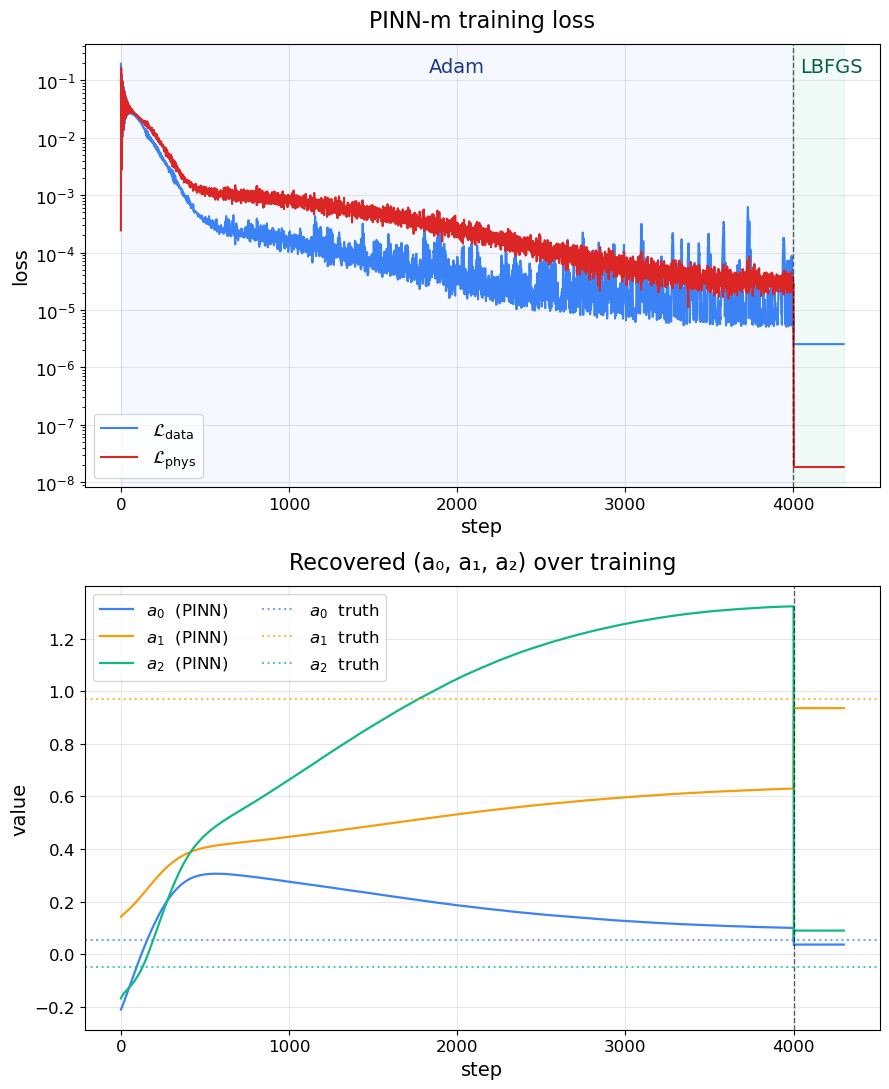
\includegraphics[width=1.05\columnwidth]{figures/training_output.png}
  \caption{Training dynamics. Top: data and physics losses on a log
  scale across the Adam$\to$L-BFGS handoff at step $4000$. Bottom:
  the three trainable scalars $(a_0, a_1, a_2)$ against their
  analytical Glauber values (dotted).}
  \label{fig:training}
\end{figure}

During the Adam phase, $a_2$ does more than miss its target: it
drifts in the wrong direction entirely, climbing toward $+1.3$ while
the true value sits near $-0.05$. The reason is a curvature mismatch between the two
optimizers. In the closed m-equation residual~\eqref{eq:residual-def}
the coefficient $a_2$ multiplies $m(t)^2$, and on the condition
shown $m(t)$ stays in $[0, 0.4]$ so $m(t)^2 \!\lesssim\! 0.16$
everywhere. The curvature corresponding to $a_2$ is therefore
small, and the loss surface along the $a_2$ direction is
correspondingly flat. Adam, being a first-order optimizer with
diagonal preconditioning, lets $a_2$ wander down that flat valley
as long as $a_0$ and $a_1$ absorb the change; the trajectory MSE
stays small but the scalars are jointly biased. L-BFGS, by contrast,
builds an explicit low-rank approximation of the curvature, picks up
the off-diagonal coupling between $(a_0, a_1, a_2)$, and snaps each
scalar onto its correct value in a single curvature-aware update.
The visible drop at step $4000$ marks the handoff between the two optimizers.
 This two-phase schedule works because the two methods address different problems:
  Adam carries the loss most of the way down, but it converges slowly along the
   stiff parameter directions where curvature is highly anisotropic. L-BFGS, 
   which builds an explicit curvature model, resolves these directions quickly
    once Adam has brought the iterate close to the minimum.


After training, the two correlators are obtained without any additional
fitting:
\begin{equation}
  \hat\eps(t) = \mhat^2,
  \label{eq:eps-from-m}
\end{equation}
which is the independent-spins approximation, and
\begin{equation}
  \hat\epstwo(t) = \frac{2}{a_2}\Bigl[\,\dot{\hat m}(t) + (1 - a_1)\hat m(t) - \tfrac{a_0}{2}\,\Bigr],
  \label{eq:eps2-inversion}
\end{equation}
which is obtained by algebraically inverting the m-equation
\eqref{eq:m-ode}. Equation~\eqref{eq:eps2-inversion} contains no closure
error: given the trained $\mhat$ and the recovered scalars, it is exact.

Two numerical hazards are worth flagging in~\eqref{eq:eps2-inversion}.
First, the inversion divides by $a_2$, which vanishes at $J = 0$ and is
small in the high-temperature system more generally; conditions with
$|a_2| < 10^{-3}$ are numerically ill-conditioned, although by the same
token the m-equation in that system is independent of $\epstwo$ and the
inversion is uninformative. Second, $\dot{\hat m}(t)$ is
evaluated by automatic differentiation of the trained network and
inherits any high-frequency noise of $\mhat$; the Softplus MLP is
smooth enough by construction that these stay well below the
closure-bias.

I benchmark four alternative PINN variants against the chosen
PINN-Analytical pipeline: three
separate PINNs (one per observable), an Inverse PINN that learns
$(\beta, h, J)$ directly, a three-channel PINN with full
supervision, and a Per-run PINN trained on un-averaged Monte Carlo
data. All five share the same MLP primitive (four hidden layers of
$64$ Softplus units), the same data, and the same Adam$\to$L-BFGS
schedule; they differ only in what the network outputs, in which
channels are data-supervised, and in which physics residuals are
enforced. The reference implementation is in
\texttt{code/variants.py}.

The three-separate-PINN design uses one network per observable. The
m-PINN takes the chosen-pipeline form: it is trained on $\mbar$ with
the closed m-equation residual~\eqref{eq:residual-def}. The
$\eps$-PINN is trained on $\bar\eps$ and enforces the
$\eps$-equation~\eqref{eq:e-ode}, with $m(t)$ and $\epstwo(t)$
supplied as external forcing from the Monte Carlo data; this needs
both companion observables, so the physics constraint is weaker than
in the chosen pipeline. The $\epstwo$-PINN has no native ODE in the
closed-moment system and is therefore a pure curve-fit on
$\bar\epstwo$. Each of the three networks carries its own copy of
$(a_0, a_1, a_2)$, so the design produces three independent and
possibly inconsistent estimates of the scalars; only the m-PINN's
scalars are reported in the benchmark. Total parameter count $38{,}028$,
roughly $3\times$ the chosen pipeline.

The Inverse PINN keeps the architecture of the chosen pipeline but
makes the trainable scalars the physical parameters $(\beta, h, J)$
rather than $(a_0, a_1, a_2)$; the Glauber forward
map~\eqref{eq:glauber-fwd} is applied at every training step to
convert those parameters into the coefficients that enter the
residual. This tests whether parameterizing through the physical
model improves identifiability of $(\beta, h, J)$ from a single
trajectory. The parameter count is $12{,}676$, matching the chosen
pipeline. The trade-off is that when $|a_2|$ is small, which happens
at $J = 0$ and in the high-temperature system, the forward
map~\eqref{eq:glauber-fwd} is nearly flat in $J$, so the optimizer
can drift along that direction with no penalty in the residual.

The chosen PINN-Analytical pipeline is a single m-PINN with output
$\mhat$ and three trainable scalars $(a_0, a_1, a_2)$, with the
two correlators recovered analytically
through~\eqref{eq:eps-from-m}-\eqref{eq:eps2-inversion} after
training. Parameter count $12{,}676$.

The three-channel PINN with full supervision uses a single MLP with
three outputs $(\mhat, \hat\eps, \hat\epstwo)$, all of which are
data-supervised on the chain-averaged and ensemble-averaged trajectories,
and a physics term that enforces both~\eqref{eq:m-ode}
and~\eqref{eq:e-ode} at residual points, with $\hat\epstwo(t)$
supplied by the network's third output rather than through a closure
assumption. This tests whether the analytical post-hoc reduction in the
chosen pipeline leaves accuracy on the table: more outputs, more
supervision, more physics. Parameter count $12{,}806$ (essentially
the same as the chosen pipeline; the three output heads add only
$\sim\!130$ parameters to the shared core). In practice the
in-domain trajectory MSE does not improve on the chosen design, and
on the extrapolation experiment of Section~\ref{sec:results} the
held-out error is substantially worse, because the fully supervised
loss locks the network to the training window without a
corresponding mechanism to propagate the dynamics beyond it.

The Per-run PINN is architecturally identical to the chosen pipeline
but is trained on a single un-averaged Monte Carlo realization
rather than on the $K = 8$ ensemble average. This isolates the role
of the physics term as a noise filter. The supervised signal is the
noisy single-realization $m(t)$ trajectory (the faint cloud
underlying the $m$-panel of Figure~\ref{fig:variants-traj} is that
data), and the physics constraint is the only mechanism that can
pull $\mhat$ onto the smooth underlying ODE solution. Parameter
count $12{,}676$.

The data pipeline that feeds the PINN is the most operationally
involved part of the framework, and its design choices materially
affect both the supervised target $\mbar$ and the validation targets
$\bar\eps(t)$, $\bar\epstwo(t)$. The simulation ingredients are
therefore described in some detail below, in the correct order.


The closed-moment ODEs in \eqref{eq:m-ode}-\eqref{eq:e-ode} are exact
under the Glauber heat-bath rule in the thermodynamic limit. They are
\emph{not} exact under single-spin-flip dynamics or under
synchronous-update schemes, because both alter the local flip rates in
ways that change the coefficients of the moment expansion. Using the
matching microscopic dynamics is therefore not the best choice but a
prerequisite for a meaningful comparison between the recovered
coefficients $(\hat a_0, \hat a_1, \hat a_2)$ and the analytical
forward map~\eqref{eq:glauber-fwd}. Any other update rule would force
the PINN to absorb a residual mismatch into the scalars and would
contaminate the inverse-problem reading of the results.


For each Monte Carlo step a spin index $i$ is drawn uniformly at
random from $\{1, \dots, N\}$. The local field at site $i$ is
$f_i = h + J(\sigma_{i-1} + \sigma_{i+1})$, evaluated with periodic
boundary conditions $\sigma_0 \!\equiv\! \sigma_N$ and
$\sigma_{N+1} \!\equiv\! \sigma_1$. The spin is then drawn from the
local conditional thermal equilibrium distribution: it is set to $+1$ with
probability $p_+ = \tfrac{1}{2}\bigl(1 + \tanh \beta f_i\bigr)$ and to
$-1$ otherwise. This rule is independent of the previous value of
$\sigma_i$, which is what makes it the heat-bath (rather than the
single-spin-flip) variant of Glauber dynamics, and is the choice for which
the closed-moment ODEs hold cleanly.

One Monte Carlo time unit is defined as $N$ such single-spin
attempts, i.e.\ one full sweep of the chain on average, so that the
natural time axis of the simulator agrees with the time axis of the
closed-moment ODE up to an $\mathcal{O}(1)$ rescaling that is
absorbed into the coefficients $(a_0, a_1, a_2)$.

\begin{figure}[H]
  \centering
  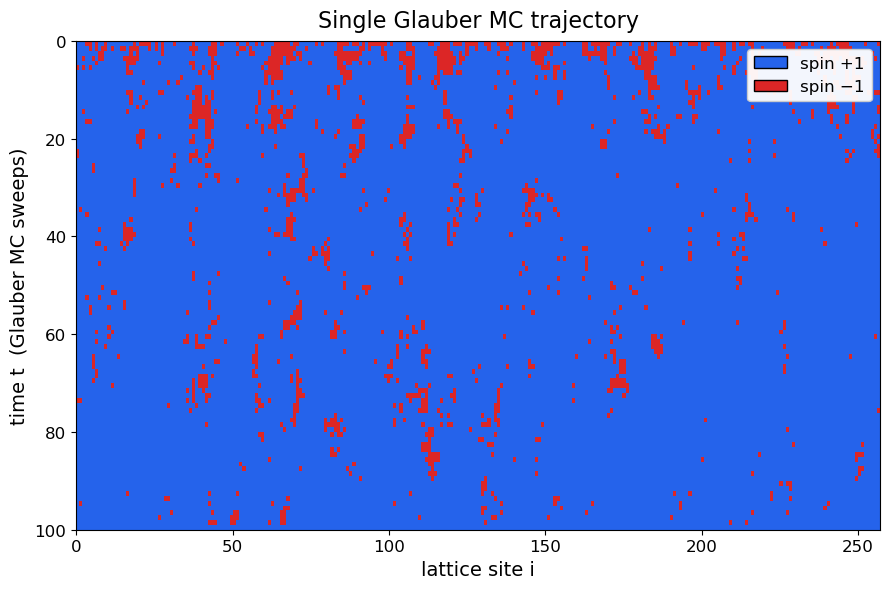
\includegraphics[width=0.85\columnwidth]{figures/data_trajectory.png}
  \caption{Single Glauber Monte Carlo realization on a $256$-spin
  chain. Blue is $+1$, red is $-1$. The chain-averaged
  helicity $\mbar$ at time $t$ is the row-mean across this map;
  the closed-moment ODE describes the dynamics of that row-mean and
  of its two short-range correlators.}
  \label{fig:trajectory}
\end{figure}

Figure~\ref{fig:trajectory} shows a single such trajectory as a
space-time map. The chain relaxes from the fully aligned initial
state, and the residual $-1$ domains form, drift, and annihilate as
the system equilibrates. The chain-and-ensemble averages of this raw
configuration field are what the closed-moment ODE describes, and
what the PINN is trained against.




The chain uses $N = 256$ spins with periodic boundary conditions. This size is
well into the system where the chain-averaged moments are quantitatively
close to the thermodynamic-limit ODE: the leading finite-size correction
to a chain-averaged single-site observable scales as $\mathcal{O}(1/N)$
in the high-temperature expansion, which here is below the noise floor
of the eight-trajectory group. Periodic boundary conditions are
chosen rather than open boundaries because the chain-average step that
produces~\eqref{eq:m-ode}-\eqref{eq:e-ode} assumes translation
invariance, which open boundaries break. I verified empirically
that doubling the chain to $N = 512$ shifts the chain-averaged
trajectories by less than the realization-to-realization standard
deviation, so $N = 256$ trades simulator time for a controlled bias.


Each realization is initialized with all spins set to $+1$, which
corresponds to a fully aligned starting state $m(0) = 1$ and
$\eps(0) = \epstwo(0) = 1$. A uniform-random initialization
($m(0) \approx 0$) was tried and gives qualitatively similar PINN
performance, but the aligned initialization is more demanding because
the system must traverse the full relaxation trajectory to reach
equilibrium, exposing the time-dependent term in the m-equation more
sharply. The full trajectory is kept: the trajectory from
$t = 0$ to $t = T$ is the object the PINN is asked to fit, including
the rapid early-time descent.


For each of the $100$ conditions on the parameter grid, eight
independent Glauber realizations are run with distinct random seeds, and
the chain-averaged moments are then averaged a second time across
realizations. The number $K = 8$ is a deliberate compromise: at
$K = 1$ the residual single-realization noise leaks into the
PINN's data loss and the residual term has to fight against it,
inflating both the helicity MSE and the recovered-coefficient
error; at $K = 32$ the data becomes smoother but the marginal benefit
is below the closure bias from the
$\epstwo \!\approx\! m^2$ approximation, so the additional simulator
cost is not justified. The $K = 8$ setting puts the data noise
roughly an order of magnitude below the closure bias, which is the
system in which the physics term is most informative.


The grid spans
$(\beta, h, J) \in \mathrm{Linspace}(0.2, 1.5, 5)
\times \mathrm{Linspace}(0.01, 0.20, 5)
\times \mathrm{Linspace}(0.5, 1.5, 4)$,
for a total of $5 \times 5 \times 4 = 100$ conditions. The temperature
range covers both the high-temperature system ($\beta = 0.2$, where
the chain is essentially uncorrelated and $a_0, a_2 \!\approx\! 0$)
and the low-temperature system ($\beta = 1.5$, where the tanh
arguments approach equilibrium and the chain is strongly correlated).
The field range is symmetric about zero so that the helicity can
be driven to either fixed point and so that any sign-asymmetry in the
recovered scalars surfaces immediately. The coupling range includes
both ferromagnetic ($J > 0$) and antiferromagnetic ($J < 0$)
systems; the latter exercises the tanh expansion in a system where
$a_0$ and $a_1$ change sign and provides a stress test for the
recovered-coefficient comparison.


Each trajectory is run for $T = 100$ Monte Carlo time units and is
sampled on a uniform grid of $99$ time points (the data array
$\bar m_i$ used in $\mathcal{L}_\text{data}$). The collocation grid
for $\mathcal{L}_\text{phys}$ is independent of the data grid: $200$
points are drawn uniformly from $[0, T]$ at each L-BFGS outer
iteration, so the residual is not evaluated at the same locations as
the data term. This separation is intentional: it prevents the network
from satisfying the residual easily by overfitting at the data
points alone, and it ensures the physics constraint is felt across the
whole interval rather than only at the data anchors.


The simulator is JIT-compiled with Numba~\cite{numba}, which brings
single-realization completion down to a few seconds at $N = 256$ and
$T = 100$, so that the full $100$-condition grid with $K = 8$
realizations completes in minutes on a single CPU core. Random seeds
are fixed per condition so that the recorded trajectories are
bit-reproducible. The chain-averaged trajectories
$(\bar m, \bar\eps, \bar\epstwo)$ are stored in a single
\texttt{.npz} archive that is consumed unchanged by all PINN variants
in the benchmark; this guarantees that variant-to-variant differences
in Section~\ref{sec:results} reflect architectural choices rather than
data-generation noise.

\section{Results}
\label{sec:results}

\begin{figure*}[!tb]
  \centering
  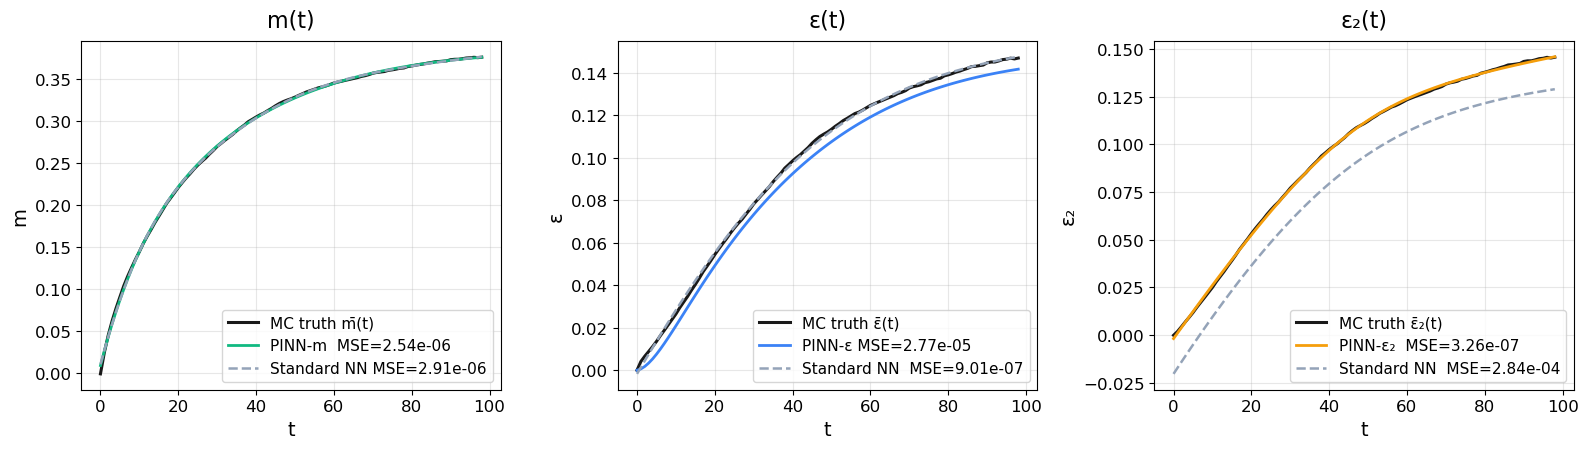
\includegraphics[width=0.9\textwidth]{figures/training_fit.png}
  \caption{In-domain fit of the PINN-Analytical pipeline against
  Monte Carlo truth on a representative condition. Left: the
  helicity $\mhat$, which is the only quantity that appears in
  the loss. Middle: the nearest-neighbor correlator $\hat\eps(t)$
  recovered from the independent-spins approximation
  \eqref{eq:eps-from-m}. Right: the next-nearest-neighbor correlator
  $\hat\epstwo(t)$ recovered analytically from the
  m-equation~\eqref{eq:eps2-inversion}; this is the only post-hoc
  step in the pipeline that is closure-free, and the residual error
  is dominated by the precision of $\mhat$ and the recovered scalars.}
  \label{fig:in-domain}
\end{figure*}

The condition shown in Figure~\ref{fig:in-domain} is drawn from the
intermediate-temperature system at moderate
positive coupling and small positive field, which sits in the
working region of the closed-moment ODE description: the
independent-spins approximation~\eqref{eq:eps-from-m} is accurate to
$\mathcal{O}(\beta J)$ here, small enough that the separation
between the two correlator estimators is clear without being
overwhelmed by closure error. The figure reports the trained PINN's
predictions for the three observables alongside the Monte Carlo
ground truth.

The helicity $\mhat$ overlays the truth to within
$\mathrm{MSE} \sim 10^{-6}$. The two correlators, recovered
analytically through~\eqref{eq:eps-from-m} and~\eqref{eq:eps2-inversion},
match the Monte Carlo trajectories to within
$\mathrm{MSE} \sim 10^{-5}$ on $\eps$ and $\mathrm{MSE} \sim 10^{-7}$
on $\epstwo$, despite neither quantity appearing in the training
loss. The agreement is visually exact at the resolution of the
panels; it is only quantitatively that the two correlators separate,
and that separation is informative about the structure of the
post-hoc reduction itself.


The next-nearest-neighbor correlator $\hat\epstwo(t)$ is fit better
than the nearest-neighbor correlator $\hat\eps(t)$, even though it
sits one step further from the supervised quantity in the moment
hierarchy. The reason is that the two correlators are
recovered by structurally different post-hoc steps. The estimator
for $\eps(t)$ in~\eqref{eq:eps-from-m} is the independent-spins
approximation $\langle \sigma_k \sigma_{k+1}\rangle \approx m^2$,
which is exact only at $\beta = 0$ and carries an irreducible
$\mathcal{O}(\beta J)$ closure error at finite temperature. No
matter how precise $\mhat$ becomes, $\hat\eps$ cannot fall below
this closure-bias floor. The estimator for $\epstwo(t)$ in
\eqref{eq:eps2-inversion}, by contrast, is an algebraic inversion of
the \emph{exact} m-equation and contains no closure step at all; its
accuracy is therefore bounded only by the precision of $\mhat$ and
of the recovered scalars, both of which sit at $\mathcal{O}(10^{-3})$
after L-BFGS convergence. So $\hat\eps$ inherits a modeling bias
that $\hat\epstwo$ does not, and that bias is the dominant
contribution to the gap between their MSEs.



The same pattern carries across the 100-condition grid. The absolute
MSE on $\hat\eps$ tracks the strength of the coupling: at small
$\beta J$ the independent-spins assumption is nearly exact and the two
correlators are fit to similar precision, while at strong $\beta J$
the closure error widens and the gap visible in
Figure~\ref{fig:in-domain} grows accordingly. The helicity MSE, by
contrast, is essentially insensitive to $\beta J$ and stays at the
$\mathcal{O}(10^{-6})$ level set by the network's capacity and the
Adam$\to$L-BFGS convergence.



At the level of trajectory shape, the helicity $\mhat$ relaxes
monotonically from the fully aligned initial value $m(0) = 1$
toward the field-biased equilibrium fixed point. The relaxation
rate is set jointly by $(1 - a_1)$, which gives the linear damping
toward equilibrium, and by $a_2/2$, which enters as a quadratic
correction once $\mhat$ moves away from its early steady-state value. The
PINN tracks both the fast initial descent and the slow late-time
approach without any explicit time-scale separation in the loss,
because the physics residual penalizes ODE violations uniformly
across collocation points sampled from the full interval $[0, T]$
rather than concentrating on any particular portion of the
relaxation trajectory.

\begin{figure}[!htb]
  \centering
  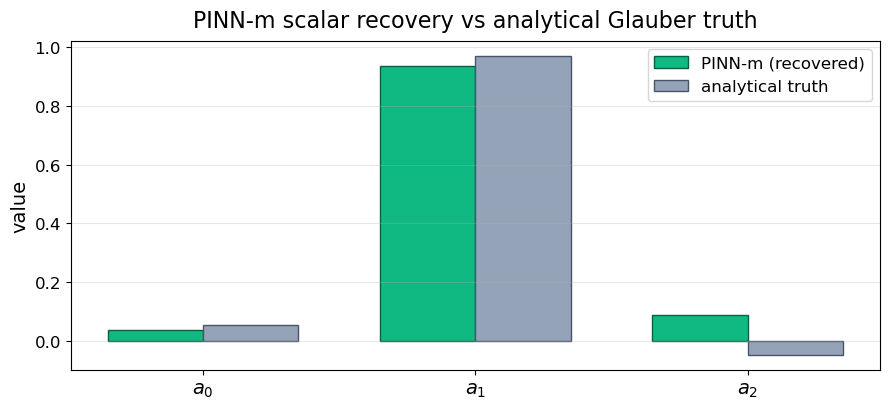
\includegraphics[width=\columnwidth]{figures/scalars_vs_standard_nn.png}
  \caption{PINN-recovered Glauber scalars compared with the
  analytical forward map. The dominant
  coefficient $a_1$ is recovered to a few percent.
  $a_0$ and $a_2$ are recovered in the correct magnitude range; the
  larger relative error on $a_2$ is consistent with its small
  contribution to the m-equation residual.}
  \label{fig:scalar-recovery}
\end{figure}

Figure~\ref{fig:scalar-recovery} compares the PINN-recovered scalars
$(a_0, a_1, a_2)$ against the analytical Glauber forward
map~\eqref{eq:glauber-fwd}. The dominant coefficient $a_1$ is recovered
to within a few percent of its analytical value. The smaller
coefficients $a_0$ and $a_2$ are recovered in the right magnitude
range but show larger relative error, consistent with the smaller
contribution they make to the m-equation residual. Across the
100-condition parameter grid, the mean absolute recovery error
$\overline{|\Delta a|}$ is on the order of $10^{-3}$.

Recovery is most accurate when each of $(a_0, a_1, a_2)$
contributes meaningfully to the m-equation residual. When $|a_2|$
is small, either at $J = 0$ or in the high-temperature system, the
loss surface flattens along the $a_2$ direction and the recovered
value of $a_2$ becomes weakly identified: the trajectory MSE on $m$
stays small but the relative error on $a_2$ can be large. The same
system is where the post-hoc
inversion~\eqref{eq:eps2-inversion} that recovers $\epstwo$
becomes ill-conditioned, since dividing by a vanishing $a_2$
amplifies any error in $\mhat$. Conditions with $|a_2| < 10^{-3}$
are flagged in the data pipeline and excluded from the
recovered-coefficient statistic above.



\begin{figure}[H]
  \centering
  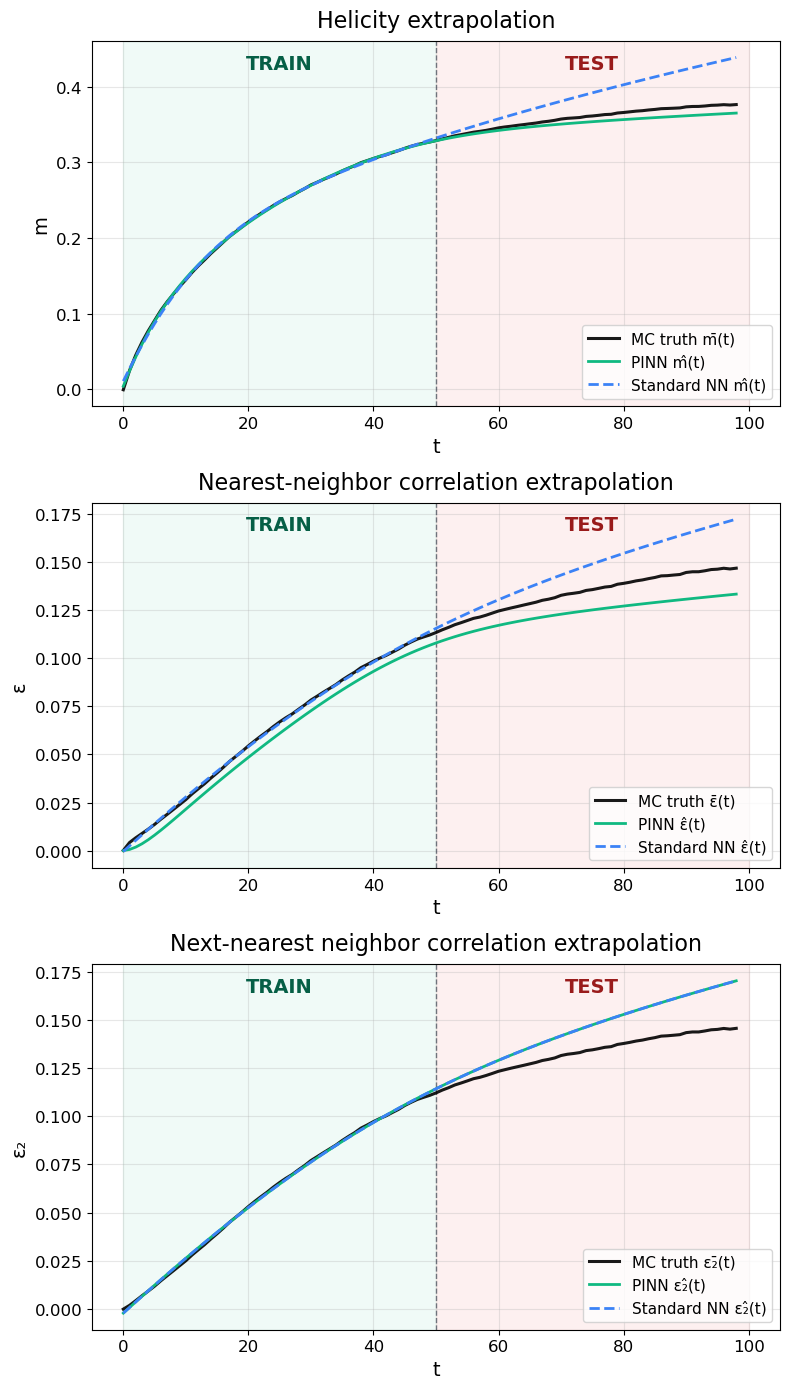
\includegraphics[width=0.95\columnwidth]{figures/extrapolation_comp.png}
  \caption{PINN vs.\ standard MLP on a 50\%/50\% train/test split.
  Both fit the training half tightly; the PINN tracks the Monte
  Carlo truth on the held-out half while the unconstrained MLP
  drifts after the training window ends.}
  \label{fig:extrapolation}
\end{figure}

With both the trajectory fit and the coefficient recovery
established on a representative condition, the natural next
question is whether the physics term confers genuine generalization
or whether the trained PINN is merely a high-precision interpolator
of the training trajectory. A clean test is to restrict the
data-loss term to a sub-interval of $[0, T]$ while keeping the
physics residual on the full window. If the residual is doing real
work, the trained network should track the Monte Carlo trajectory
on the held-out portion as well; if it is not, the network should
behave like an unconstrained MLP and drift off once the supervised
window ends.


To test whether the physics term confers genuine generalization
beyond in-domain interpolation, I train the same architecture on the
first half of each trajectory ($t \in [0, T/2]$) and evaluate on the
held-out second half. The PINN remains close to the Monte Carlo truth
on the held-out interval, while a vanilla MLP baseline trained
without the physics term drifts off as soon as the training window
ends. Figure~\ref{fig:extrapolation} compares the two on the three
observables, and Figure~\ref{fig:extrapolation-mse} reduces that
comparison to a single joint MSE summed over $m$, $\eps$, and
$\epstwo$ on the held-out half: the PINN sits roughly an order of
magnitude below the standard-NN baseline. The split is chosen to be
aggressive (50\%/50\%) so that the test interval is genuinely
out-of-window rather than a nearby neighborhood of the training
data, which would not separate a physics-constrained network from
an interpolating one.

The standard-NN baseline fails in a specific way on the held-out
half. Its predictions continue along the trend of the training
data without any restoring force, so they drift monotonically off
the Monte Carlo trajectory as soon as $t > T/2$. The PINN's
predictions stay bound to the closed-moment ODE through the
residual term, which is evaluated on collocation points sampled
uniformly from the full interval $[0, T]$ and therefore continues
to penalize ODE violations on the test half even though no
supervised data are available there. The order-of-magnitude gap in
joint test MSE between the two is the size of that anchoring
effect for this representative condition.

\begin{figure}[H]
  \centering
  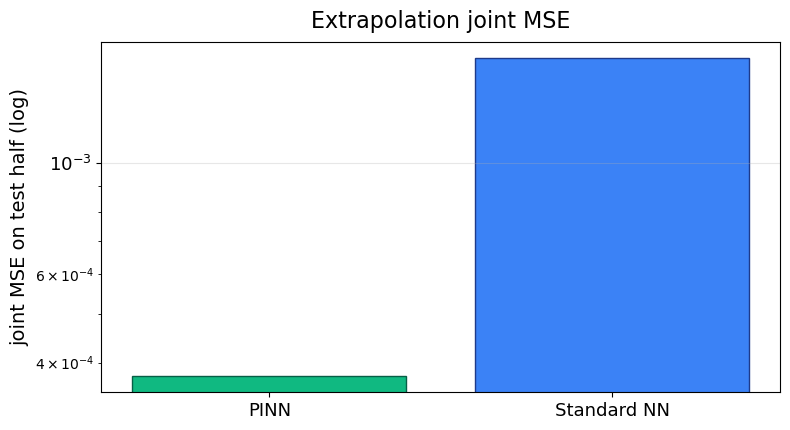
\includegraphics[width=0.85\columnwidth]{figures/joint_MSE__Extrapol.png}
  \caption{Joint test MSE (sum over $m$, $\eps$, $\epstwo$) on the
  held-out half of the trajectory. The PINN's joint extrapolation
  MSE is roughly an order of magnitude below the standard-NN
  baseline.}
  \label{fig:extrapolation-mse}
\end{figure}

The contrast is sharper when the held-out comparison is collapsed
to a single scalar per network. Figure~\ref{fig:extrapolation-mse}
reports the joint MSE summed over the three observables on the
held-out half, on a logarithmic axis chosen so that the
order-of-magnitude separation between the two networks is clear.
The bars confirm what the trajectory panels of
Figure~\ref{fig:extrapolation} already suggested visually: the two
networks reach essentially identical accuracy on the training
half, and the entire difference between them lives in the held-out
region. The same pattern persists across the parameter grid. The
standard-NN extrapolation MSE scales with the held-out trajectory
length, growing roughly linearly with the size of the unsupervised
interval, while the PINN's held-out MSE stays close to its
in-domain value because the residual term continues to anchor the
network where no supervised data is available. This is the
clearest signature, on this condition, that the physics loss is
contributing more than a regularizer effect.



\begin{figure}[H]
  \centering
  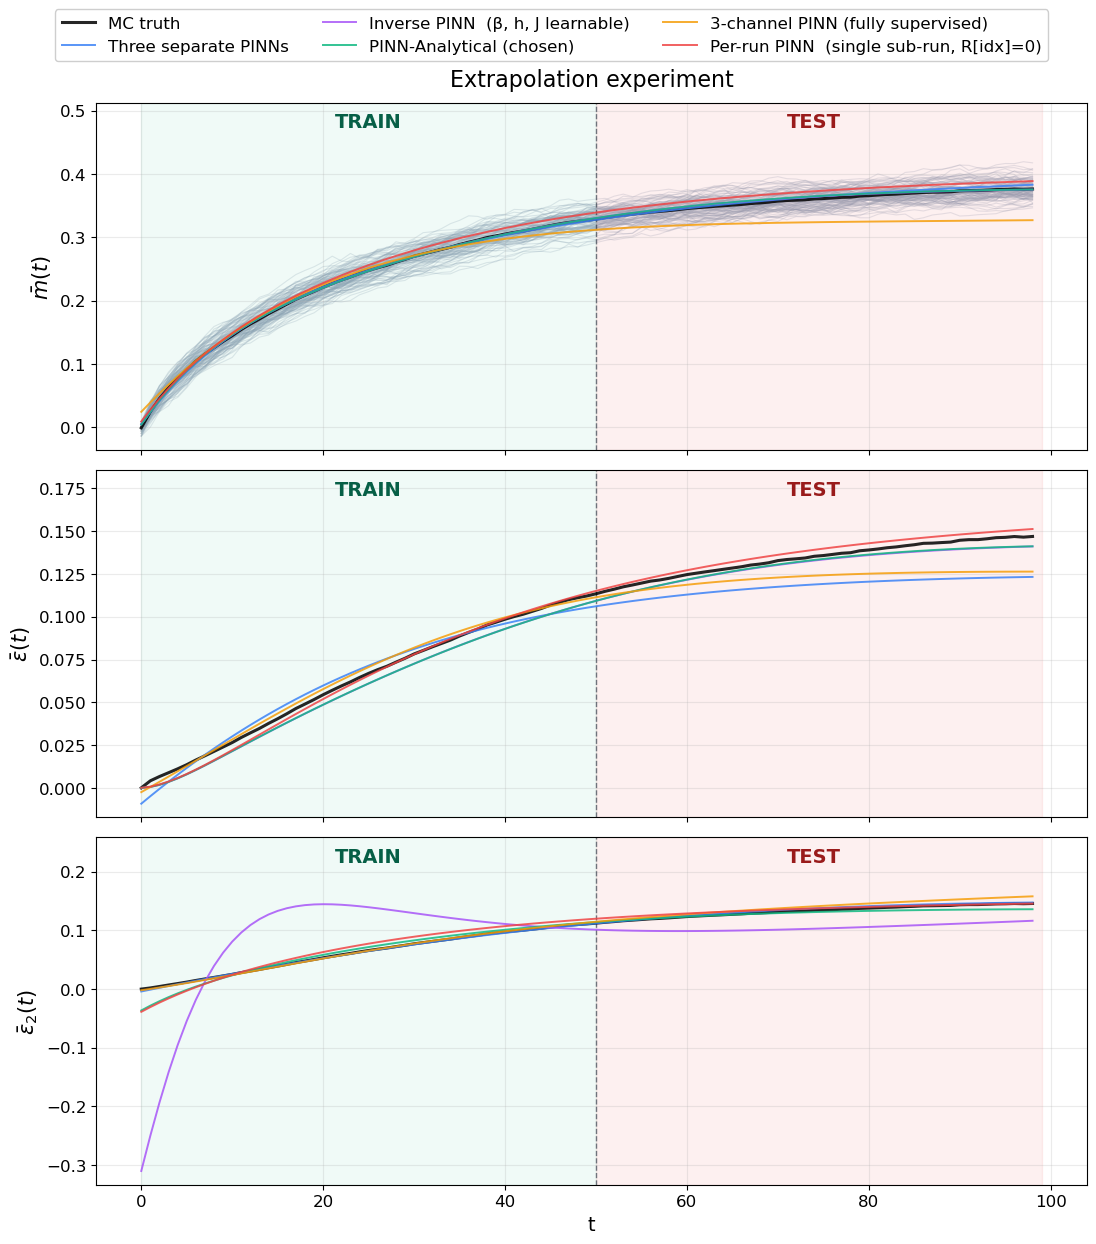
\includegraphics[width=0.9\columnwidth]{figures/extrapolation_experiment.png}
  \caption{Five PINN variants on the 50\%/50\% extrapolation split.
  From top to bottom: $m(t)$, $\eps(t)$, $\epstwo(t)$. The
  PINN-Analytical (chosen) trajectory is the only one that is
  closure-free in $\epstwo$ and is competitive on the other two
  observables.}
  \label{fig:variants-traj}
\end{figure}

The same 50\%/50\% split lets each of the five PINN variants be
held to the same standard. All variants share identical MLP
primitives and the identical Adam$\to$L-BFGS schedule (see
\texttt{benchmarks.ipynb}), so any difference between them traces
back to the loss-side choices catalogued earlier. Figure
\ref{fig:variants-traj} reports the trajectories of $m(t)$,
$\eps(t)$, and $\epstwo(t)$ across the train/test split for each
variant. The 3-channel PINN (orange) overfits the training half
but drifts visibly on the held-out half because its fully
supervised loss is not tied to the closed-moment ODE; the other
variants stay close to the Monte Carlo curves.

\begin{figure}[H]
  \centering
  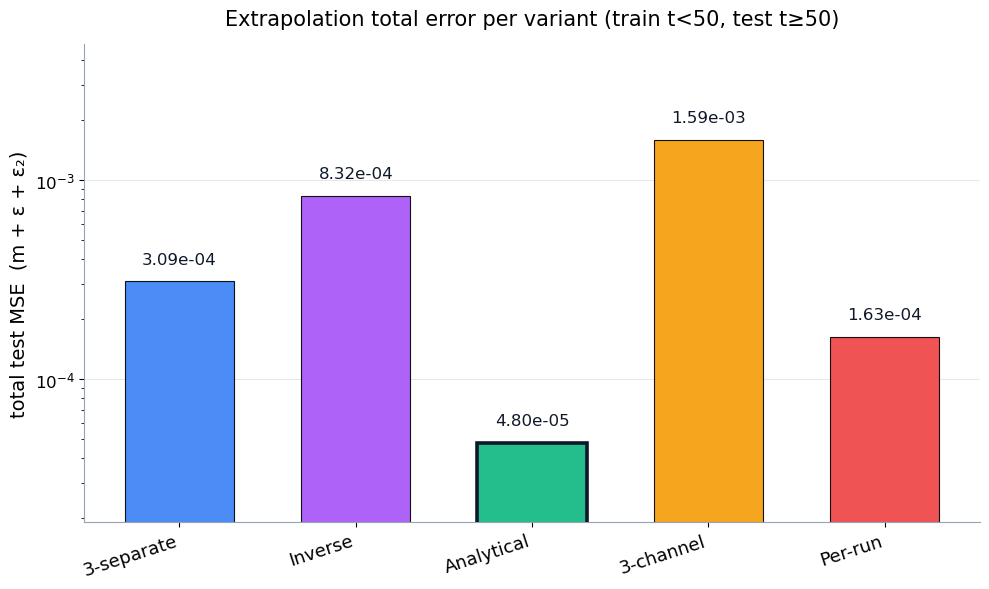
\includegraphics[width=0.85\columnwidth]{figures/extrapolation_error_1.png}
  \caption{Total extrapolation MSE per variant (sum over $m$,
  $\eps$, $\epstwo$ on the held-out half). The chosen
  PINN-Analytical pipeline (green) is the lowest.}
  \label{fig:variants-mse}
\end{figure}

\noindent Figure~\ref{fig:variants-mse} summarizes each variant by a
single scalar: the total held-out MSE across the three observables.
PINN-Analytical achieves $4.8 \times 10^{-5}$, an order of magnitude
better than Per-run ($1.6 \times 10^{-4}$) and two orders of magnitude
better than the 3-channel baseline.

Evaluating the same per-variant comparison on a separately
generated dataset with more negative coupling and field $(J, h)$
(Figure~\ref{fig:variants-mse-m}) preserves the ranking,
indicating that the chosen pipeline's advantage is not tied to the
original parameter grid. The Inverse PINN, which trains
$(\beta, h, J)$ as latent variables and recovers the scalars
through the Glauber forward map~\eqref{eq:glauber-fwd}, sits in
the middle of the pack and shows the weakened identifiability
that motivates avoiding the forward-map composition in the chosen
design.

\begin{figure}[H]
  \centering
  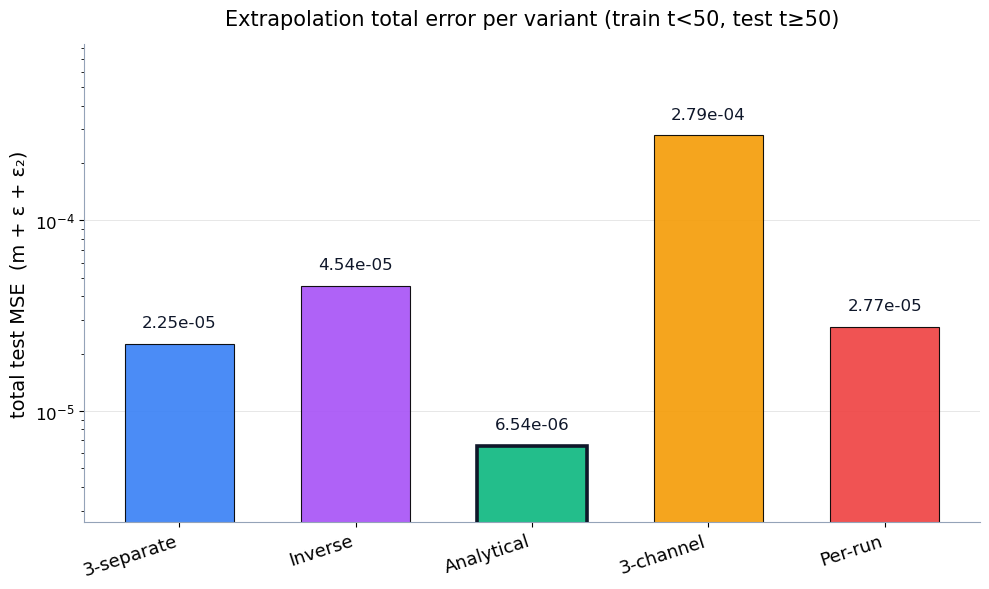
\includegraphics[width=0.8\columnwidth]{figures/extrapolation_error_2.png}
  \caption{Same per-variant comparison as
  Figure~\ref{fig:variants-mse}, evaluated on a separately
  generated dataset with more negative coupling and field values
  ($J, h$).}
  \label{fig:variants-mse-m}
\end{figure}

\section{Analysis and Validation}
\label{sec:analysis}


The closed-moment system has two ODEs in three unknowns. Choosing which
observable to learn first is therefore a real design decision, not a
notational convenience. I probe this choice by training the same
architecture on the m-equation, on the $\eps$-equation, and as a
curve-fit on $\bar\epstwo(t)$. The corresponding experiment
(\texttt{alternative\_observables.ipynb}) shows that only the m-equation
closes under a tractable approximation: the $\eps$-equation requires
both $m(t)$ and $\epstwo(t)$ as external forcing, weakening the physics
constraint, and $\epstwo$ has no native ODE in the closed-moment system.
Coefficient recovery degrades correspondingly. This validates $m$ as the
natural starting observable for the framework.


Monte Carlo is the natural ground truth, but it is also useful as a cost
baseline. Generating one $T = 100$ trajectory at $N = 256$ spins,
averaged over $8$ realizations, requires on the order of seconds in
the JIT-compiled simulator. PINN inference, by contrast, requires a single
forward pass through a $\sim 13{,}000$-parameter MLP, which is several
orders of magnitude faster. The PINN therefore acts as a fast surrogate
once trained, with the additional benefit that its predictions are
constrained to satisfy the closed-moment ODE.


The chosen pipeline has three limitations worth noting.
First, the independent-spins closure $\epstwo \approx m^2$ used inside
the m-equation residual is exact only at infinite temperature; for finite
$\beta$ it introduces a small systematic bias whose magnitude grows in
the strongly coupled system. Second, the framework is condition-specific:
each $(\beta, h, J)$ requires its own training run. A multi-condition
extension that learns a shared core is left for future work.
Third, the underlying chain is one-dimensional, where the closed-moment
expansion is particularly clean; the same approach in two or three
dimensions would require either higher-order moment closures or a return
to the full configurational state.

\section{Discussion and Conclusion}
\label{sec:conclusion}

I have presented a PINN framework that learns the dynamics of an
Ising-like Zimm-Bragg chain by embedding the closed-moment Glauber
ODE directly in the training loss of a small multilayer perceptron. The
chosen pipeline trains only on the helicity $\mbar$ and recovers
the full set of three observables $(\mhat, \hat\eps, \hat\epstwo)$
together with the underlying Glauber coefficients $(a_0, a_1, a_2)$.
The two correlators are derived analytically from the trained
$\mhat$, with no additional networks or supervision.

Across a 100-condition grid, the network reproduces the Monte Carlo
trajectories at $\mathrm{MSE}$ on the order of $10^{-7}$ on the
helicity and matches the analytical Glauber forward map to within
$\sim\!10^{-3}$ on the recovered coefficients. A head-to-head benchmark
against four alternative PINN designs (separate-channel, inverse,
3-channel, per-run) confirms that the analytical post-hoc reduction is
the most parameter-efficient and most stable of the candidates.

Future work includes extension to a multi-condition shared-core
architecture, application to two and three-dimensional Ising chains
where the closed-moment expansion does not terminate at low order, and
direct application to experimental polypeptide melting data, where the
model could serve as a fast inverse-problem solver for the underlying
Zimm-Bragg parameters.

\FloatBarrier

\appendices

\section{Derivation of the closed-moment Glauber ODEs}
\label{app:moment-ode}

This appendix derives the system
\eqref{eq:m-ode}-\eqref{eq:e-ode} from the microscopic master
equation. The argument follows the line of reasoning of
Glauber~\cite{glauber1963} and the helix-coil kinetics derivation
of Allahverdyan et al.~\cite{allahverdyan2009kinetics}, specialized
to the heat-bath rule used in the simulator and made compact for
the one-dimensional chain.


Let $P(\boldsymbol{\sigma}, t)$ denote the probability of finding the
chain in configuration $\boldsymbol{\sigma} = (\sigma_1, \dots, \sigma_N)$
at time $t$. Single-spin-flip Glauber dynamics evolve $P$ according to
\begin{equation}
  \frac{\partial P(\boldsymbol{\sigma}, t)}{\partial t}
    = \sum_{i=1}^{N} \bigl[\,
        w_i(\boldsymbol{\sigma}^{(i)}) P(\boldsymbol{\sigma}^{(i)}, t)
        - w_i(\boldsymbol{\sigma}) P(\boldsymbol{\sigma}, t)
      \bigr],
  \label{eq:master}
\end{equation}
where $\boldsymbol{\sigma}^{(i)}$ is the configuration with spin $i$
flipped and $w_i(\boldsymbol{\sigma})$ is the rate at which $\sigma_i$
flips given the current configuration. The heat-bath rule
$p(\sigma_i \!\to\! +1) = \tfrac{1}{2}(1 + \tanh \beta f_i)$ corresponds
to a flip rate
\begin{equation}
  w_i(\boldsymbol{\sigma}) = \tfrac{1}{2}\bigl[\,1 - \sigma_i \tanh \beta f_i\,\bigr],
  \label{eq:flip-rate}
\end{equation}
with local field $f_i = h + J(\sigma_{i-1} + \sigma_{i+1})$.


Multiplying~\eqref{eq:master} by $\sigma_k$ and summing over all
configurations gives the standard result that, for any single-spin
observable,
\begin{equation}
  \frac{d}{dt}\langle \sigma_k \rangle
    = -2 \langle \sigma_k\, w_k(\boldsymbol{\sigma}) \rangle.
  \label{eq:single-spin}
\end{equation}
Substituting~\eqref{eq:flip-rate} into~\eqref{eq:single-spin},
\begin{equation}
  \frac{d}{dt}\langle \sigma_k \rangle
    = -\langle \sigma_k \rangle + \langle \tanh \beta f_k \rangle.
  \label{eq:m-pre-expand}
\end{equation}
The remaining task is to evaluate $\langle \tanh \beta f_k \rangle$.


The local field $f_k$ depends on $(\sigma_{k-1}, \sigma_{k+1})$, which
takes only four values, but $\sigma_{k-1} + \sigma_{k+1}$ takes only
three: $+2$, $0$, $-2$. Writing the indicator algebra
$\delta_{S=+2} = \tfrac{1}{4}(1+\sigma_{k-1})(1+\sigma_{k+1})$ etc.\
and substituting,
\begin{align}
  \tanh\beta f_k
    &= A + B(\sigma_{k-1} + \sigma_{k+1}) + C\,\sigma_{k-1}\sigma_{k+1}, \nonumber \\
  A &= \tfrac{1}{4}\bigl[\tanh\beta(h+2J) + 2\tanh\beta h + \tanh\beta(h-2J)\bigr], \nonumber \\
  B &= \tfrac{1}{4}\bigl[\tanh\beta(h+2J) - \tanh\beta(h-2J)\bigr], \label{eq:tanh-expand} \\
  C &= \tfrac{1}{4}\bigl[\tanh\beta(h+2J) - 2\tanh\beta h + \tanh\beta(h-2J)\bigr]. \nonumber
\end{align}
The three coefficients $(2A, 2B, 2C)$ are exactly $(a_0, a_1, a_2)$ in
\eqref{eq:glauber-fwd}. Substituting~\eqref{eq:tanh-expand} into
\eqref{eq:m-pre-expand} and chain-averaging yields
\begin{equation}
  \dot m = -m + a_0/2 + a_1 m + (a_2/2)\,\langle \sigma_{k-1}\sigma_{k+1}\rangle,
\end{equation}
which is~\eqref{eq:m-ode} after recognizing
$\epstwo = \langle \sigma_{k-1}\sigma_{k+1}\rangle$ as the
next-nearest-neighbor correlator. The companion equation
\eqref{eq:e-ode} is derived analogously, starting from
$d\langle \sigma_k \sigma_{k+1}\rangle/dt$.

\section{Derivation of the physics loss}
\label{app:phys-loss}

This appendix records how the physics term $\mathcal{L}_\text{phys}$
in \eqref{eq:l-phys} is obtained from the closed-moment ODE.


The closed m-equation~\eqref{eq:m-ode-closed} can be written in
residual form by moving every term to one side:
\begin{equation}
  R_m(t) := \dot m(t) + \bigl(1 - a_1\bigr) m(t)
            - \tfrac{a_0}{2} - \tfrac{a_2}{2}\,m(t)^2.
  \label{eq:residual-def-app}
\end{equation}
A function $m(\cdot)$ is a solution of \eqref{eq:m-ode-closed} on
$[0,T]$ if and only if $R_m(t) \equiv 0$ for all $t \in [0,T]$. The
PINN replaces this pointwise zero condition with a sampled
mean-square objective, which is the standard PINN
construction~\cite{raissi2019pinn} and is the residual definition
shown in~\eqref{eq:l-phys} when $\hat m$ replaces the unknown $m$ and
the trainable scalars $(a_0, a_1, a_2)$ replace the
analytical Glauber coefficients.


The time derivative $\dot{\hat m}(t_{c,j})$ in
$\mathrm{Res}_m(t_{c,j})$ is obtained by backpropagating through 
the network with respect to its scalar input
$t$, evaluated at the collocation point $t_{c,j}$. There are
two implementation details.

First, the smooth Softplus activation in the MLP is what makes this
derivative useful: a ReLU network has a piecewise-constant first
derivative, whose samples are visited by the residual loss
at each batch and produce a non-smooth model that
defeats the L-BFGS line search. Second, the collocation points
$t_{c,j}$ are resampled at each L-BFGS outer iteration; this is
technically a Monte Carlo estimator of the integral of
$R_m^2$, and resampling reduces its variance.


The residual~\eqref{eq:residual-def-app} hides one closure step: the
exact m-equation~\eqref{eq:m-ode} contains $\epstwo(t)$, which has
been replaced by $m(t)^2$. This is the independent-spins approximation
$\langle \sigma_{k-1}\sigma_{k+1}\rangle \approx \langle \sigma_k \rangle^2$,
which is exact at $\beta = 0$ and is asymptotic at high temperature;
its leading-order correction is
$\mathcal{O}(\beta J)$, which sets the lower bound on the achievable residual error.
This approximation enters only inside the residual that
drives training; the analytical post-hoc step in
Appendix~\ref{app:eps-recovery} recovers $\epstwo(t)$ without it.


Combining the supervised data term~\eqref{eq:l-data} and the residual
term~\eqref{eq:l-phys},
\begin{equation}
  \mathcal{L}_\text{total}
    = \underbrace{\frac{1}{N_d} \sum_{i=1}^{N_d}
        \bigl(f_\theta(t_i) - \bar m_i\bigr)^2}_{\mathcal{L}_\text{data}}
      + \underbrace{\frac{1}{N_c} \sum_{j=1}^{N_c}
        R_m(t_{c,j})^2}_{\mathcal{L}_\text{phys}},
  \label{eq:total-loss}
\end{equation}
where $\bar m_i = \mbar[t_i]$ is the chain-and-ensemble averaged
Monte Carlo helicity at sampling time $t_i$. No separate
weighting hyperparameter is introduced between the two terms: in
this setup both $\mathcal{L}_\text{data}$ and $\mathcal{L}_\text{phys}$
sit at comparable magnitudes by the end of the Adam phase, and
L-BFGS is run on the unweighted sum.

\section{Recovering $\eps(t)$ and $\epstwo(t)$ from $m(t)$}
\label{app:eps-recovery}


The PINN does not directly target $\eps(t)$, so it is estimated from
$\mhat$ alone. Under the independent-spins approximation,
\begin{equation}
  \langle \sigma_k \sigma_{k+1} \rangle
  \approx \langle \sigma_k \rangle \langle \sigma_{k+1} \rangle
  = m^2,
  \label{eq:eps-indep-spins}
\end{equation}
which gives the estimator $\hat\eps(t) = \mhat^2$ used
in~\eqref{eq:eps-from-m}. For the high and intermediate-temperature
conditions on the parameter grid it is accurate to $\mathrm{MSE} \sim 10^{-5}$.
Strictly speaking it is the only step in the post-hoc reduction that
is not closure-free, and so it is the dominant systematic error in
$\hat\eps(t)$.


By contrast, $\epstwo(t)$ is recovered \emph{without} any
closure assumption. Returning to the exact m-equation
\eqref{eq:m-ode},
\begin{equation}
  \dot m + (1 - a_1)\,m - \tfrac{a_0}{2}
    = \tfrac{a_2}{2}\,\epstwo,
\end{equation}
which is solved algebraically for $\epstwo$:
\begin{equation}
  \epstwo(t)
    = \frac{2}{a_2}\Bigl[\,\dot m(t) + (1 - a_1)\,m(t) - \tfrac{a_0}{2}\,\Bigr].
  \label{eq:eps2-from-m-exact}
\end{equation}
Replacing the analytical $m$ and coefficients with their PINN
estimates yields~\eqref{eq:eps2-inversion}. Equation
\eqref{eq:eps2-from-m-exact} contains no approximation: given any
trajectory $m(t)$ that satisfies~\eqref{eq:m-ode} together with the
correct scalars, this expression returns the exact $\epstwo(t)$.
Its accuracy in practice is therefore determined entirely by how
faithfully $\mhat$ tracks $\mt$ and how cleanly the trainable scalars
match the analytical Glauber coefficients in~\eqref{eq:glauber-fwd}.


Two numerical hazards are worth flagging. First, the
inversion~\eqref{eq:eps2-from-m-exact} divides by $a_2$, which
vanishes at $J = 0$ and is small in the high-temperature system more
generally. Conditions with $|a_2| < 10^{-3}$ are therefore numerically
ill-conditioned, but they are also exactly the conditions under which
the m-equation is independent of $\epstwo$, so the inversion is
useful only away from this boundary. Second, the time derivative
$\dot{\hat m}(t)$ in~\eqref{eq:eps2-inversion} is evaluated by
automatic differentiation of the trained network, and inherits any
high-frequency noise of the trained $\mhat$. In practice this is
not an issue: the Softplus MLP is smooth by construction, and the
$\mhat$ trajectories obtained after L-BFGS convergence have
irregularities in $\dot{\hat m}(t)$ well below the closure-bias.

\bibliographystyle{IEEEtran}
\bibliography{references}

\end{document}
